\documentclass[a4paper,12pt,twoside,openright]{book}
\setlength\parindent{1.2em}
\setlength{\headheight}{27.11469pt}

\usepackage[final=true]{../../common/naps62}

\setlength\parindent{1.5em}

% set footnote font size to 8pt (scriptsize for class 12pt)
\let\oldfootnotesize\footnotesize
\renewcommand*{\footnotesize}{\oldfootnotesize\scriptsize}

% set line spacing to 1.5
\usepackage{setspace}
\onehalfspacing

\newcommand{\common}[1]{\input{../../common/#1}}
\newcommand{\image}[4][]{%
  \begin{figure}[!htp]%
    \centering%
    \includegraphics[#1]{#2}%
    \caption{#3 \label{#4}}%
  \end{figure}
}

\lstset{%
  tabsize=4,
  basicstyle=\footnotesize
}

% include custom mathematical definitions
\common{equations/defs}

\hypersetup{pdfauthor={Miguel Branco Palhas}}
\hypersetup{pdftitle={Thesis: An Evaluation of the GAMA/StarPU Frameworks for Heterogeneous Platforms: The Progressive Photon Mapping Algorithm}}

\addbibresource{../../common/bib/parallel.bib}
\addbibresource{../../common/bib/gama.bib}
\addbibresource{../../common/bib/starpu.bib}
\addbibresource{../../common/bib/gpu.bib}
\addbibresource{../../common/bib/verbal.bib}
\addbibresource{../../common/bib/photon_mapping.bib}

\begin{document}

\pdfbookmark{Cover}{cover}
\pagenumbering{roman}

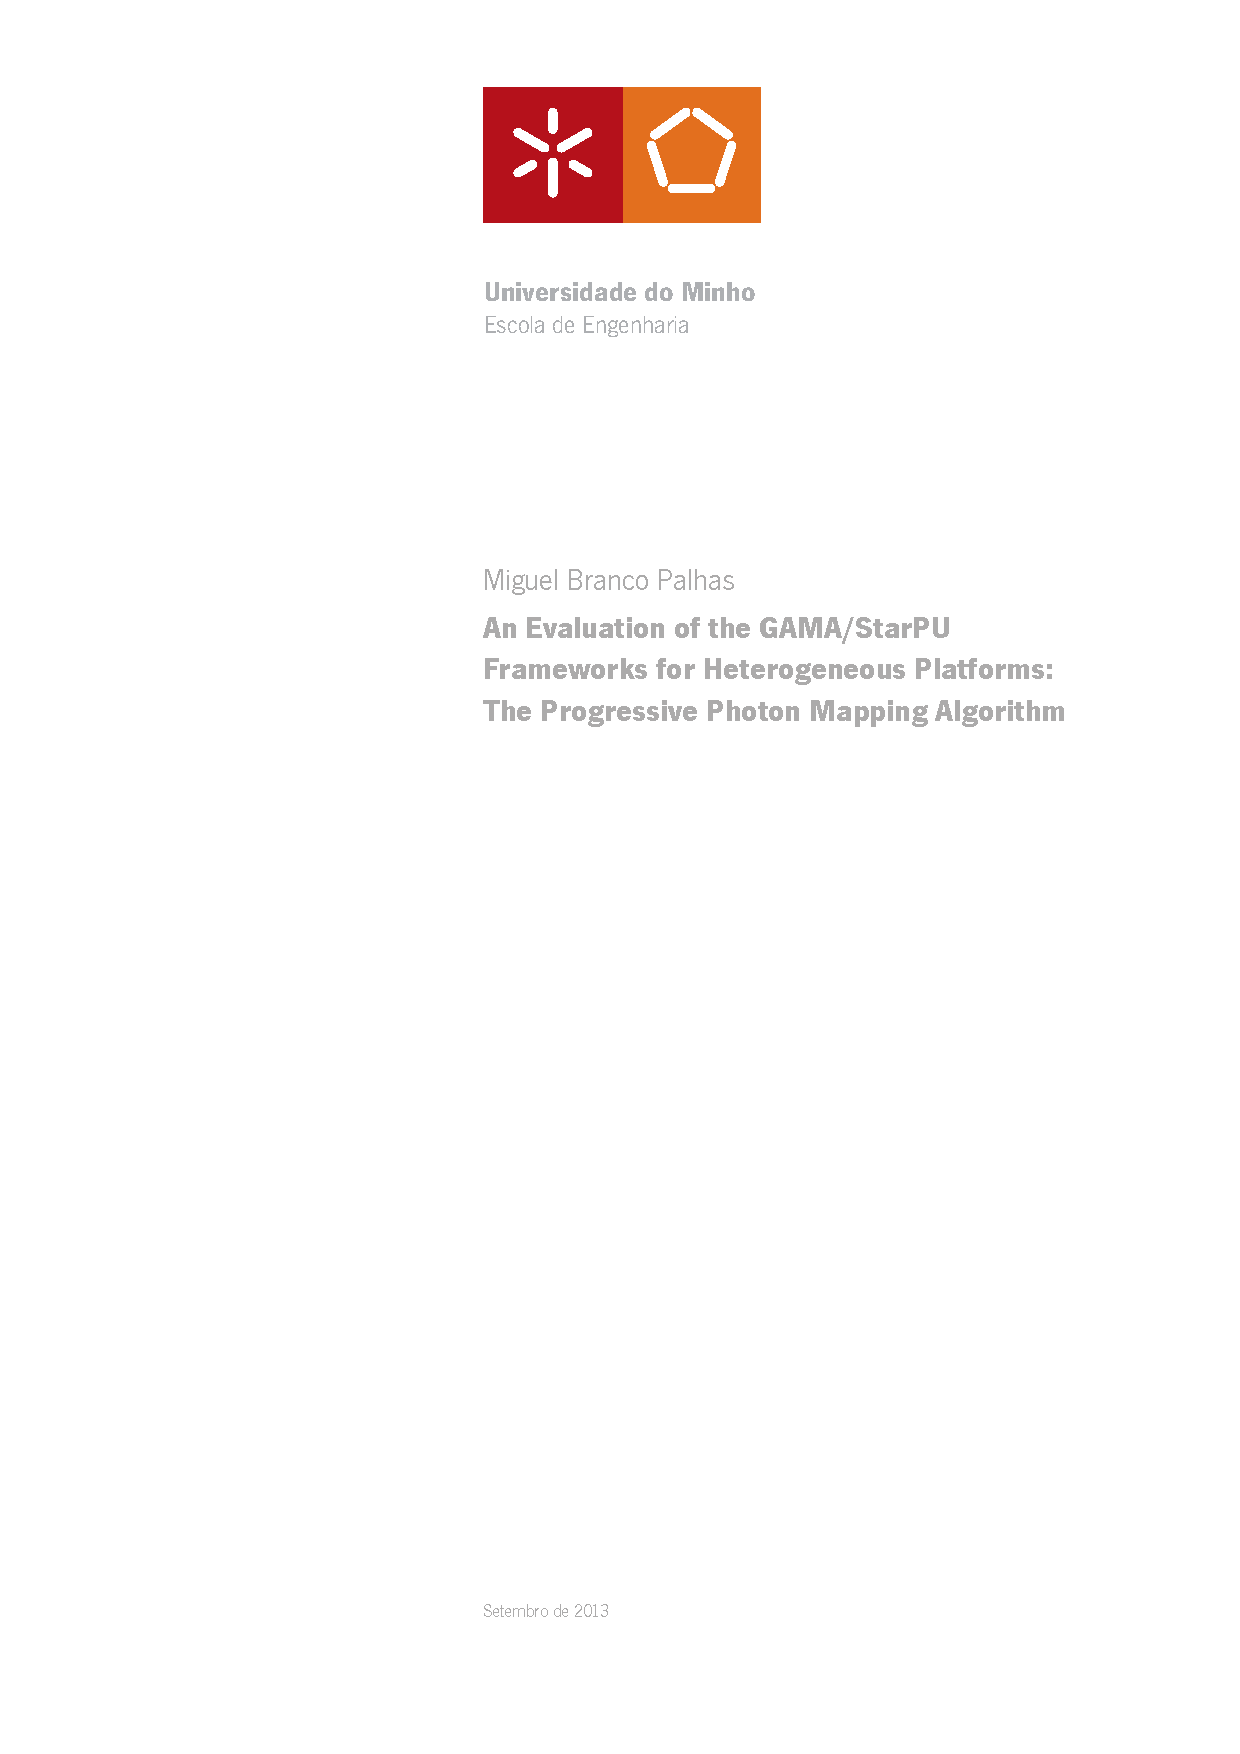
\includepdf[pages=-]{img/cover}
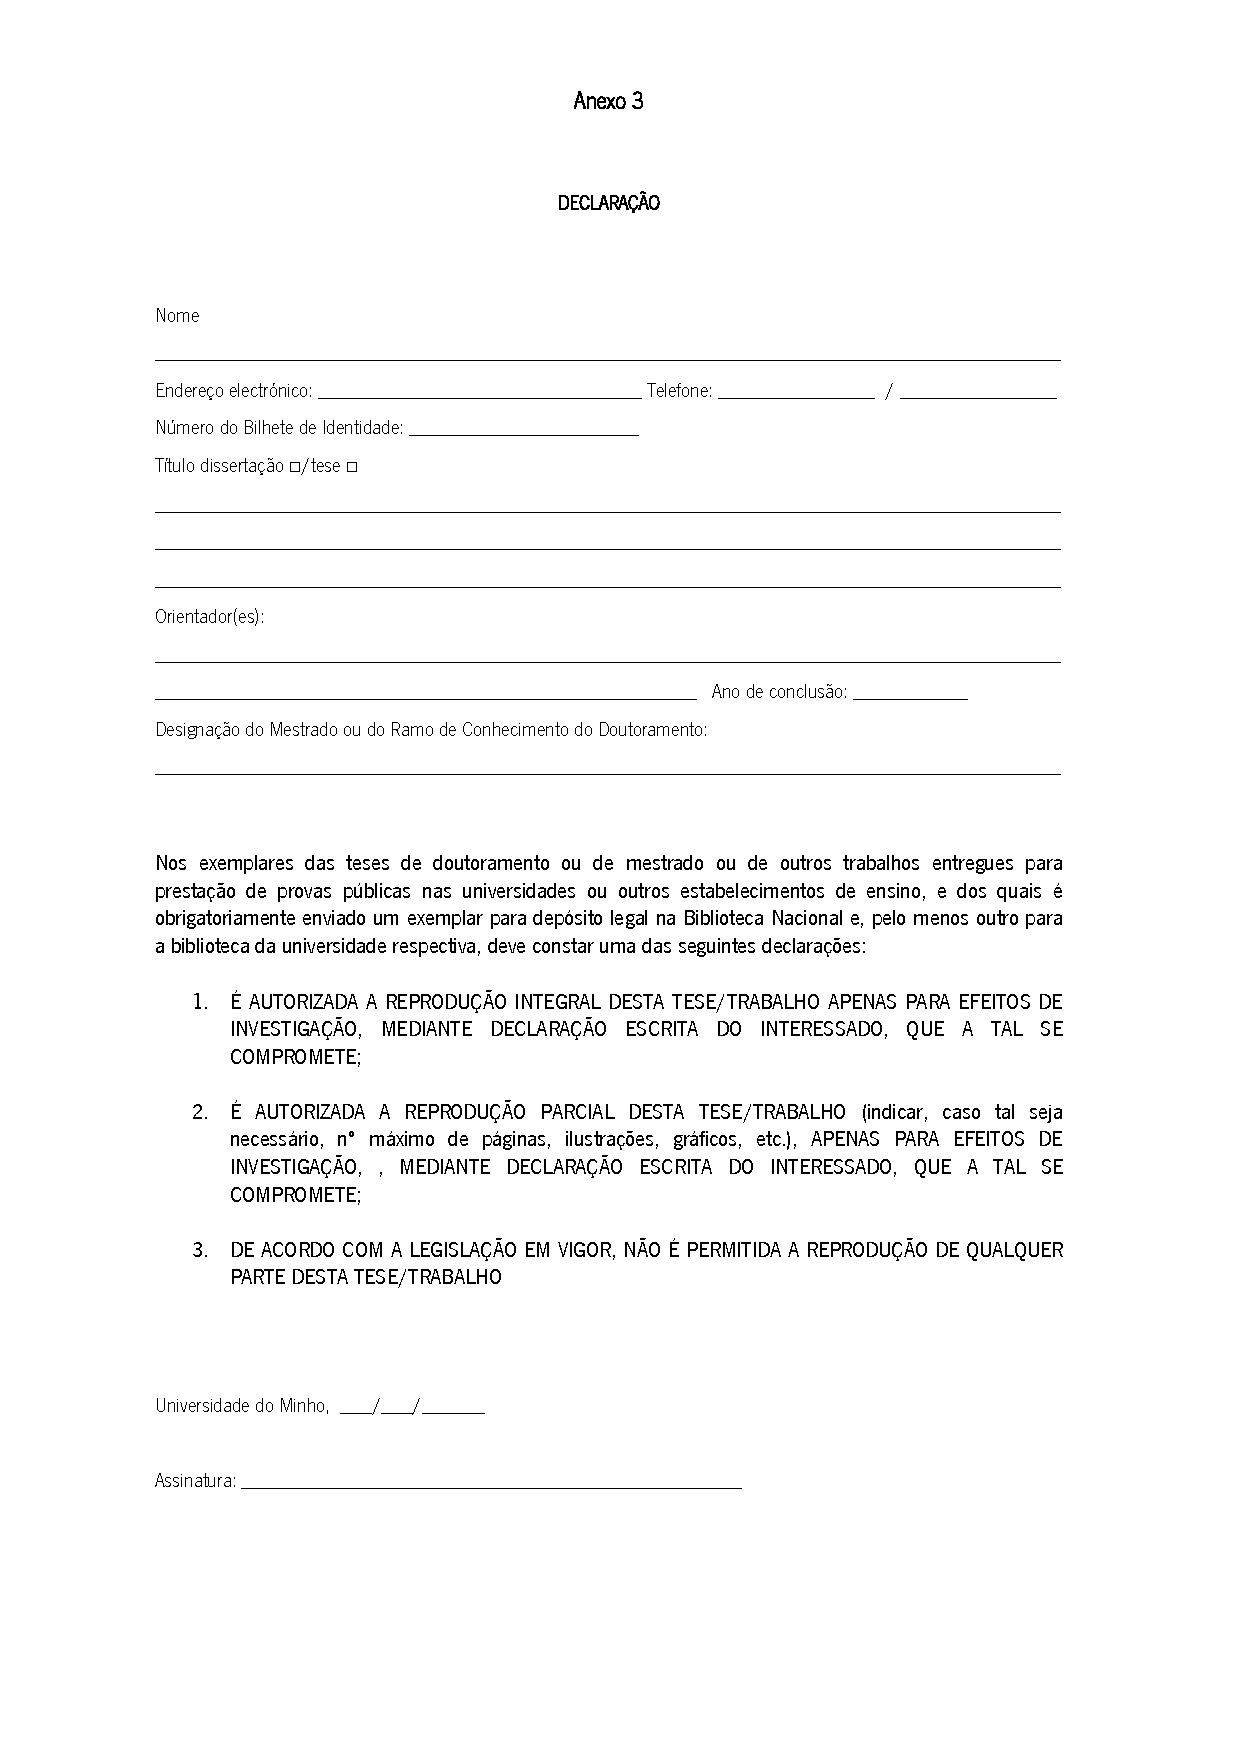
\includepdf[pages=-]{../bureaucracy/Despacho_RT-32_2005_anexoIII}

\pagestyle{fancy}
\renewcommand{\headrulewidth}{0.4pt}
\fancyhead[LO,RE]{}
\fancyhead[LE]{\slshape \leftmark}
\fancyhead[RO]{\slshape \rightmark}
\fancyfoot[RO,LE]{\thepage}%
\fancyfoot[C]{}

\fancypagestyle{plain}{%
  \renewcommand{\headrulewidth}{0.0pt}
  \fancyhead{}
  \fancyfoot[C]{}
  \fancyfoot[RO,LE]{\thepage}
}

\frontmatter
\setcounter{page}{3}
\subfile{frontmatter/01_acknowledgments}
\subfile{frontmatter/02_abstract}
\subfile{frontmatter/03_resumo}
\subfile{frontmatter/04_contents}

\cleardoublepage
\pagenumbering{arabic}

\setlength{\parskip}{1em}
\mainmatter
\subfile{tex/100_introduction}
\subfile{tex/200_background}
\subfile{tex/300_het_frameworks}
\subfile{tex/500_ppm}
\subfile{tex/600_implementation}
\subfile{tex/700_results}
\subfile{tex/800_conclusions}


\cleardoublepage
\backmatter
\pdfbookmark{References}{references}
\printbibliography
\appendix
\subfile{appendix/Z_signatures}

\end{document}
